\documentclass[tikz,border=6pt]{standalone}
\usepackage[T1]{fontenc}
\usepackage{lmodern,amsmath,amssymb}
\usetikzlibrary{arrows.meta,calc,positioning}
\definecolor{ink}{HTML}{1E293B}
\definecolor{blue}{HTML}{2563EB}
\definecolor{teal}{HTML}{0F766E}
\definecolor{red}{HTML}{A51C30}
\begin{document}
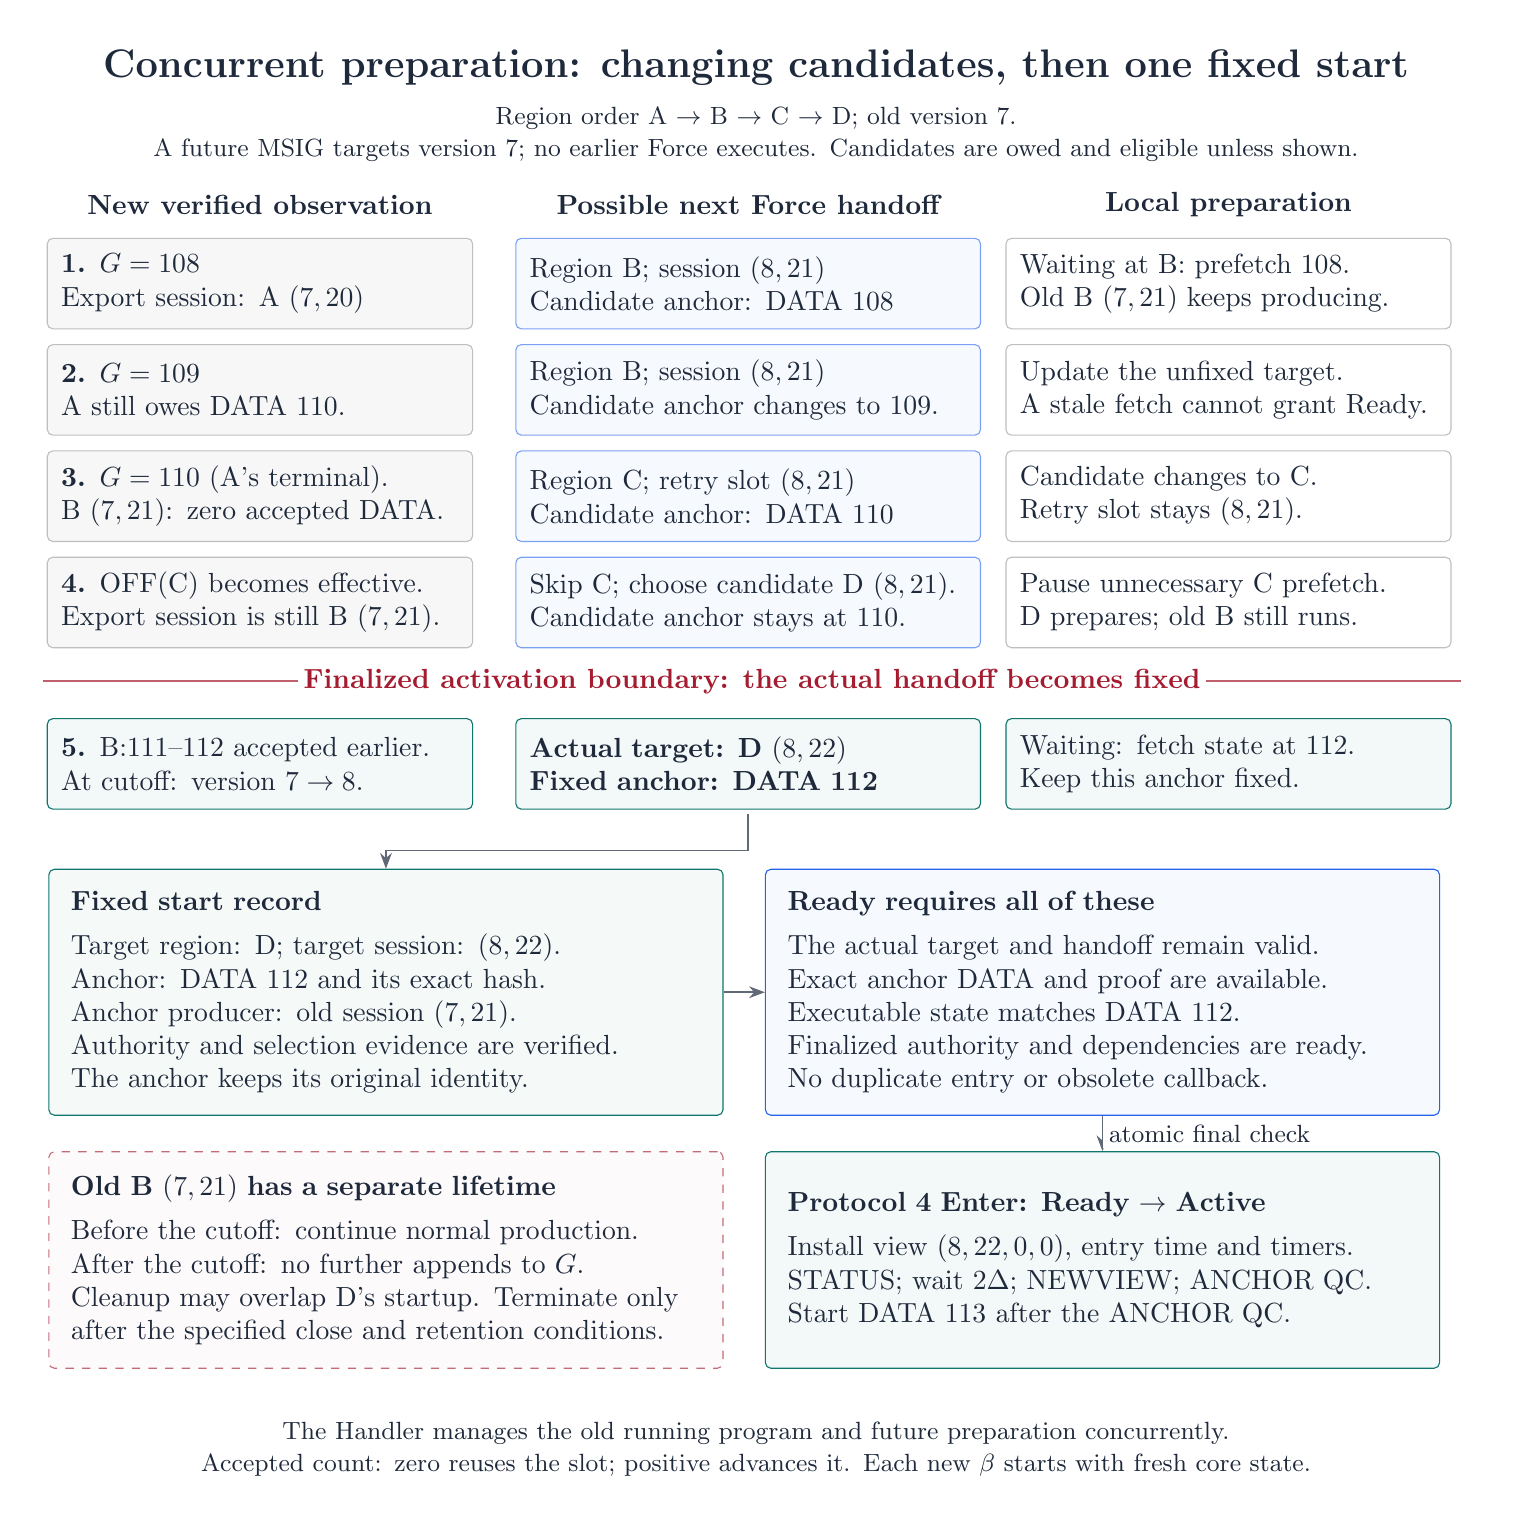
\begin{tikzpicture}[
 x=1cm,y=-1cm,font=\fontsize{10}{12}\selectfont,text=ink,
 cell/.style={draw=black!25,rounded corners=2pt,align=left,inner sep=5pt,minimum height=1.15cm},
 info/.style={cell,fill=black!3,text width=5.05cm},
 plan/.style={cell,draw=blue!60,fill=blue!4,text width=5.55cm},
 act/.style={cell,text width=5.3cm},
 box/.style={cell,text width=8.0cm,inner sep=8pt},
 flow/.style={-{Stealth[length=2mm]},semithick,draw=ink!70},
 lab/.style={fill=white,inner sep=2pt,font=\fontsize{9}{11}\selectfont,align=center}
]
\path[use as bounding box] (0,-.5) rectangle (18.5,18.3);
\node[font=\fontsize{14}{17}\selectfont\bfseries,align=center] at (9.25,0)
 {Concurrent preparation: changing candidates, then one fixed start};
\node[align=center,text width=17.6cm,font=\fontsize{9.5}{11.5}\selectfont] at (9.25,.85)
 {Region order A $\to$ B $\to$ C $\to$ D; old version 7.\\
 A future MSIG targets version 7; no earlier Force executes. Candidates are owed and eligible unless shown.};
\node[font=\bfseries] at (2.95,1.75) {New verified observation};
\node[font=\bfseries] at (9.15,1.75) {Possible next Force handoff};
\node[font=\bfseries] at (15.25,1.75) {Local preparation};

\node[info] at (2.95,2.75) {\textbf{1.} $G=108$\\Export session: A $(7,20)$};
\node[plan] at (9.15,2.75) {Region B; session $(8,21)$\\Candidate anchor: DATA 108};
\node[act] at (15.25,2.75) {Waiting at B: prefetch 108.\\Old B $(7,21)$ keeps producing.};

\node[info] at (2.95,4.1) {\textbf{2.} $G=109$\\A still owes DATA 110.};
\node[plan] at (9.15,4.1) {Region B; session $(8,21)$\\Candidate anchor changes to 109.};
\node[act] at (15.25,4.1) {Update the unfixed target.\\A stale fetch cannot grant Ready.};

\node[info] at (2.95,5.45) {\textbf{3.} $G=110$ (A's terminal).\\B $(7,21)$: zero accepted DATA.};
\node[plan] at (9.15,5.45) {Region C; retry slot $(8,21)$\\Candidate anchor: DATA 110};
\node[act] at (15.25,5.45) {Candidate changes to C.\\Retry slot stays $(8,21)$.};

\node[info] at (2.95,6.8) {\textbf{4.} OFF(C) becomes effective.\\Export session is still B $(7,21)$.};
\node[plan] at (9.15,6.8) {Skip C; choose candidate D $(8,21)$.\\Candidate anchor stays at 110.};
\node[act] at (15.25,6.8) {Pause unnecessary C prefetch.\\D prepares; old B still runs.};

\draw[draw=red!70,semithick] (.2,7.8)--(18.2,7.8);
\node[lab,text=red,font=\fontsize{10}{12}\selectfont\bfseries] at (9.2,7.8)
 {Finalized activation boundary: the actual handoff becomes fixed};

\node[info,draw=teal,fill=teal!5] at (2.95,8.85) {\textbf{5.} B:111--112 accepted earlier.\\At cutoff: version $7\to8$.};
\node[plan,draw=teal,fill=teal!5] at (9.15,8.85) {\textbf{Actual target: D $(8,22)$}\\\textbf{Fixed anchor: DATA 112}};
\node[act,draw=teal,fill=teal!5] at (15.25,8.85) {Waiting: fetch state at 112.\\Keep this anchor fixed.};

\node[box,draw=teal,fill=teal!4,minimum height=2.95cm] (fixed) at (4.55,11.75)
 {\textbf{Fixed start record}\\[4pt]
 Target region: D; target session: $(8,22)$.\\
 Anchor: DATA 112 and its exact hash.\\
 Anchor producer: old session $(7,21)$.\\
 Authority and selection evidence are verified.\\
 The anchor keeps its original identity.};
\node[box,draw=blue,fill=blue!4,minimum height=2.95cm] (ready) at (13.65,11.75)
 {\textbf{Ready requires all of these}\\[4pt]
 The actual target and handoff remain valid.\\
 Exact anchor DATA and proof are available.\\
 Executable state matches DATA 112.\\
 Finalized authority and dependencies are ready.\\
 No duplicate entry or obsolete callback.};
\draw[flow] (9.15,9.48)--(9.15,9.95)--(4.55,9.95)--(fixed.north);
\draw[flow] (fixed.east)--(ready.west);

\node[box,draw=red!65,dashed,fill=red!2,minimum height=2.75cm] (old) at (4.55,15.15)
 {\textbf{Old B $(7,21)$ has a separate lifetime}\\[4pt]
 Before the cutoff: continue normal production.\\
 After the cutoff: no further appends to $G$.\\
 Cleanup may overlap D's startup. Terminate only\\
 after the specified close and retention conditions.};
\node[box,draw=teal,fill=teal!5,minimum height=2.75cm] (active) at (13.65,15.15)
 {\textbf{Protocol 4 Enter: Ready $\to$ Active}\\[4pt]
 Install view $(8,22,0,0)$, entry time and timers.\\
 STATUS; wait $2\Delta$; NEWVIEW; ANCHOR QC.\\
 Start DATA 113 after the ANCHOR QC.};
\draw[flow] (ready.south)--node[lab,right] {atomic final check}(active.north);

\node[align=center,text width=17.4cm,font=\fontsize{9.5}{11.5}\selectfont] at (9.25,17.55)
 {The Handler manages the old running program and future preparation concurrently.\\
 Accepted count: zero reuses the slot; positive advances it. Each new $\beta$ starts with fresh core state.};
\end{tikzpicture}
\end{document}
